\input templates/header
\title[DS - BFT]{\textbf{Distributed Algorithms}\\Practical Byzantine Fault Tolerance}


\newcommand{\Retreat}{\textsc{retreat}}

\newcommand{\Request}{\textsc{request}}
\newcommand{\Preprepare}{\textsc{pre-prepare}}
\newcommand{\Prepare}{\textsc{prepare}}
\newcommand{\Commit}{\textsc{commit}}
\newcommand{\Reply}{\textsc{commit}}
\newcommand{\Checkpoint}{\textsc{checkpoint}}
\newcommand{\ViewChange}{\textsc{view-change}}
\newcommand{\NewView}{\textsc{new-view}}

\newcommand{\Prepared}{\mathbf{prepared}}
\newcommand{\Committed}{\mathbf{committed}}




\begin{document}



%-------------------------------------------------------------------------
\begin{frame}
\titlepage

{\footnotesize
Acknowledgment: Lorenzo Alvisi
}

\invisible{
\nobibliography*{references}
}

\end{frame}




%%%%%%%%%%%%%%%%%%%%%%%%%%%%%%%%%%%%%%%%%%%%%%%%%%%%%%%%%%%%%%%%%%%%%%%%%%
\section{Beyond PBFT}

\subsection{Overview}

\begin{frame}{Overview}
	
After PBFT, several others papers started to appear:
\BIL
\item \textbf{HQ}: \bibentry{hq}
\item \textbf{Q/U}: \bibentry{qu}
\EIL

The end results has been to complicate the adoption of Byzantine solutions.

\end{frame}

\begin{frame}{Overview}

\BIL
\item “In the regions we studied (up to $f=5$), if contention is low and low
latency is the main issue, then if it is acceptable to use $5f + 1$ replicas,
Q/U is the best choice, else HQ is the best since it outperforms PBFT with a
batch size of 1.”
\item “Otherwise, PBFT is the best choice in this region: It can handle high
contention workloads, and it can beat the throughput of both HQ and Q/U
through its use of batching.”
\item “Outside of this region, we expect HQ will scale best: HQ's throughput
decreases more slowly than Q/U's (because of the latter's larger message and
processing costs) and PBFT's (where eventually batching cannot compen- sate
for the quadratic number of messages).”
\EIL

\end{frame}

\section{Zyzzyva}

\subsection{Introduction}

\begin{frame}{Zyzzyva\footnote{Zyzzyva is the last word of the English dictionary}}
	
\begin{block}{OSDI'06}
{\small
\bibentry{zyzzyva}
}
\end{block}	
	
\begin{columns}
\begin{column}{0.4\textwidth}
\BIL
\item One protocol to rule them all!
\item Is Zyzzyva the last word on BFT?
\item (Or not?)
\EIL
\end{column}
\begin{column}{0.6\textwidth}
\begin{figure}
	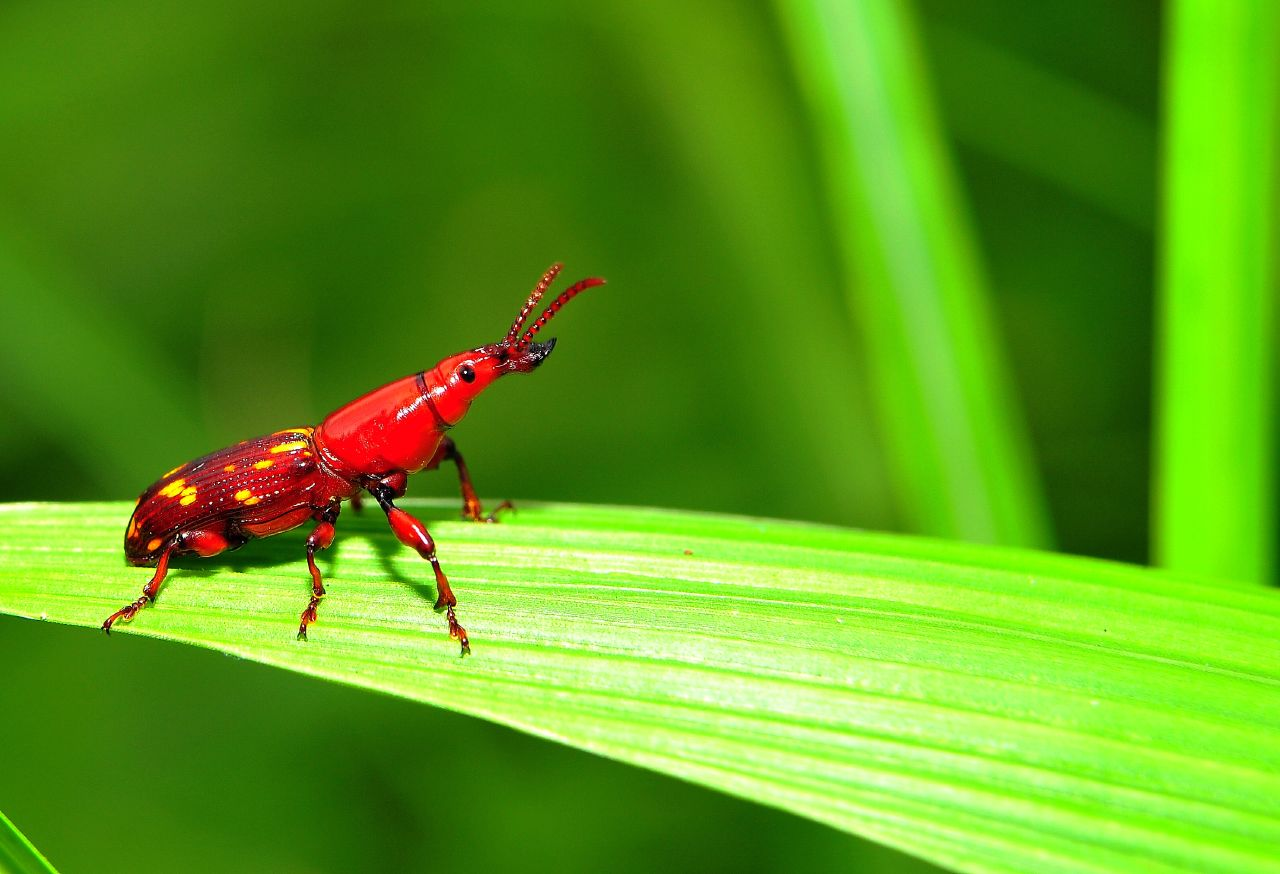
\includegraphics[width=0.6\textwidth]{figs/17/zyzzyva.png}\\
	{\tiny \url{http://www.flickr.com/photos/matthewfch/2478230533/}}
\end{figure}
\end{column}
\end{columns}

\end{frame}

\begin{frame}{Replica coordination}

\BIL
\item All correct replicas execute the same sequence of commands
\item For each received command $c$, correct replicas: 
\BI
\item Agree on $c$'s position in the sequence 
\item Execute $c$ in the agreed upon order 
\item Reply to the client	
\EI
\EIL

\end{frame}

\begin{frame}{How it is done now}
	
\begin{figure}
	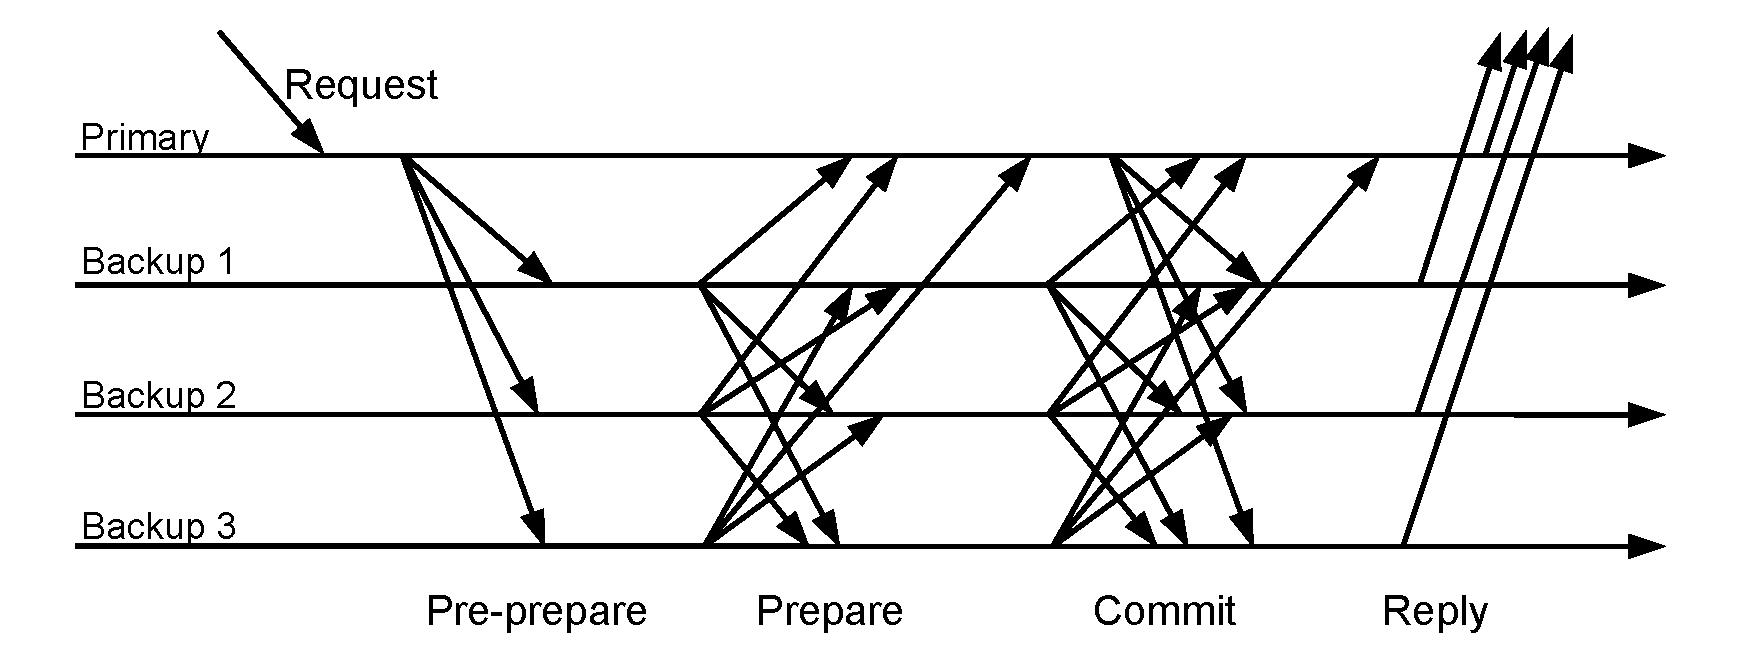
\includegraphics[width=\textwidth]{figs/17/messages4}
\end{figure}	
	
\end{frame}

\begin{frame}{The engineer's Rule of thumb}
	
\begin{block}{Citation}
\begin{quote}
Handle normal and worst case separately as a rule, because the requirements for the two are quite different:
the normal case must be fast; the worst case must make some progress
\end{quote}
Butler Lampson, “Hints for Computer System Design”
\end{block}

\end{frame}

\begin{frame}{How Zyzzyva does it}
	
\begin{figure}
	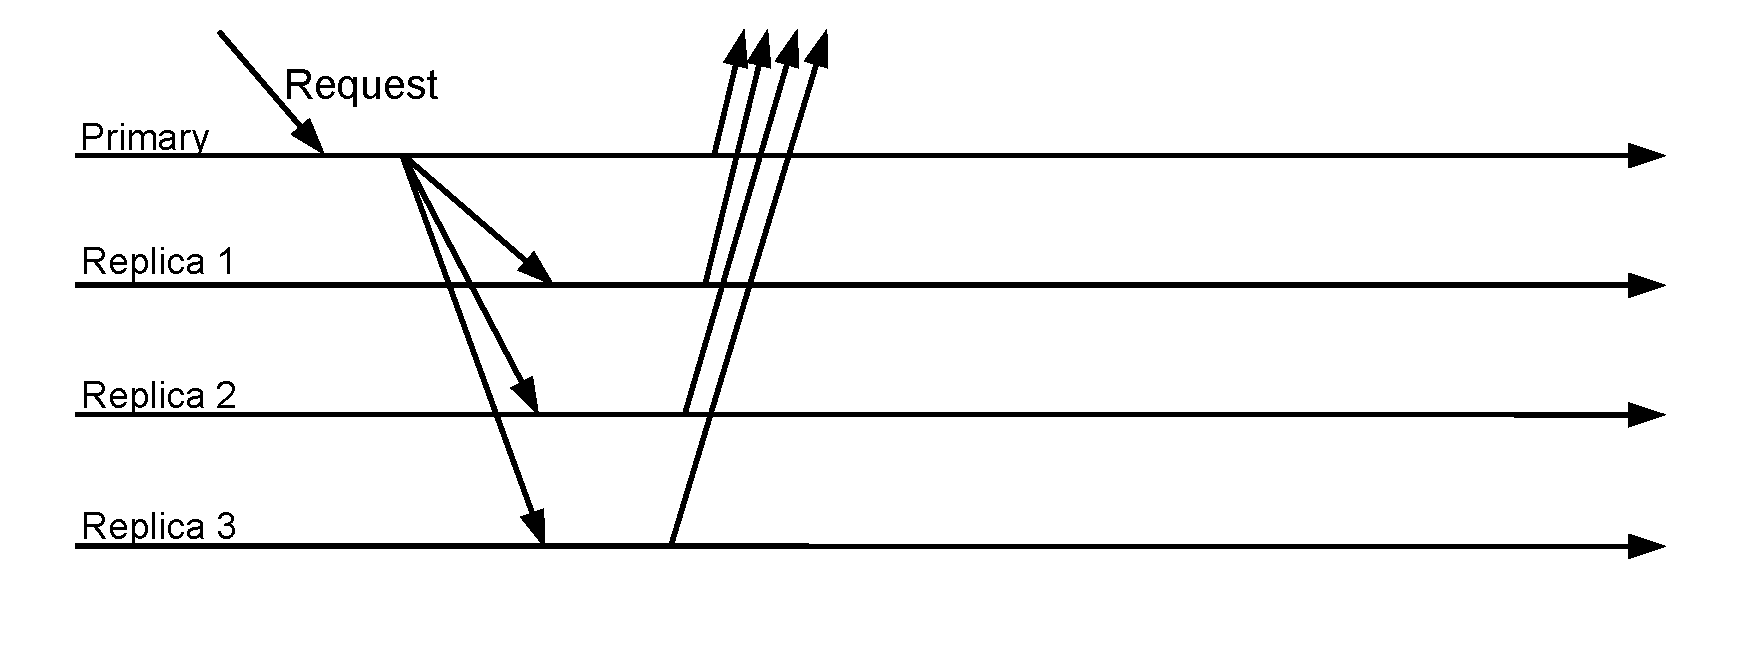
\includegraphics[width=\textwidth]{figs/17/messages5}
\end{figure}	
	
\end{frame}

\begin{frame}{Specification for State Machine Replication}

\begin{block}{Stability}
A command is \alert{stable} at a replica once its position in the sequence cannot change
\end{block}

\smallskip
\begin{block}{Safety}
Correct clients only process replies to stable commands
\end{block}

\begin{block}{Liveness}
All commands issued by correct clients eventually become stable and elicit a reply
\end{block}

\end{frame}

\begin{frame}{Enforncing safety}
\BIL
\item Safety requires:
	\BI
	\item Correct \alert{clients} only process replies to stable commands
	\EI
\item ...but RSM implementations enforce instead:
\BI
\item Correct \alert{replicas} only execute and reply to commands that are stable
\EI
\item  Service performs an output commit with each reply
\EIL
\end{frame}

\begin{frame}{Speculative BFT (Trust, but verify)}

\BIL
\item  Replicas execute and reply to a command without knowing whether it is stable
	\BI
	\item trust order provided by primary 
	\item no explicit replica agreement!
	\EI
\item Correct client, before processing reply, verifies that it corresponds to stable command
	\BI
	\item if not, client takes action to ensure liveness	
	\EI	
\EIL
	
\end{frame}

\begin{frame}{Verifying stability}
	
\BIL
\item Necessary condition for stability in Zyzzyva:
\BI
\item A command $c$ can become stable only if a majority of correct replicas
agree on its position in the sequence
\EI
\item Client can process a response for $c$ iff: 
\BI
\item a majority of correct replicas agrees on $c$'s position
\item the set of replies is incompatible, for all possible future executions,
with a majority of correct replicas agreeing on a different command holding
$c$'s current position
\EI
\EIL

\end{frame}

\begin{frame}{History}

\BIL
\item \alert{History $H_{i,k}$} is the sequence of the first $k$ commands executed by
replica $i$

\item On receipt of a command $c$ from the primary, replica appends $c$ to its
command history 
\item Replica reply for $c$ includes: 
	\BI
	\item the application-level response
	\item the corresponding command history
	\EI
\item Additional details:
	\BI
	\item Can be hashed through \alert{incremental hashing}
	\EI

\EI

\end{frame}

\subsection{Three cases}

\begin{frame}{Case 1: Unanimity}
	
\begin{figure}
	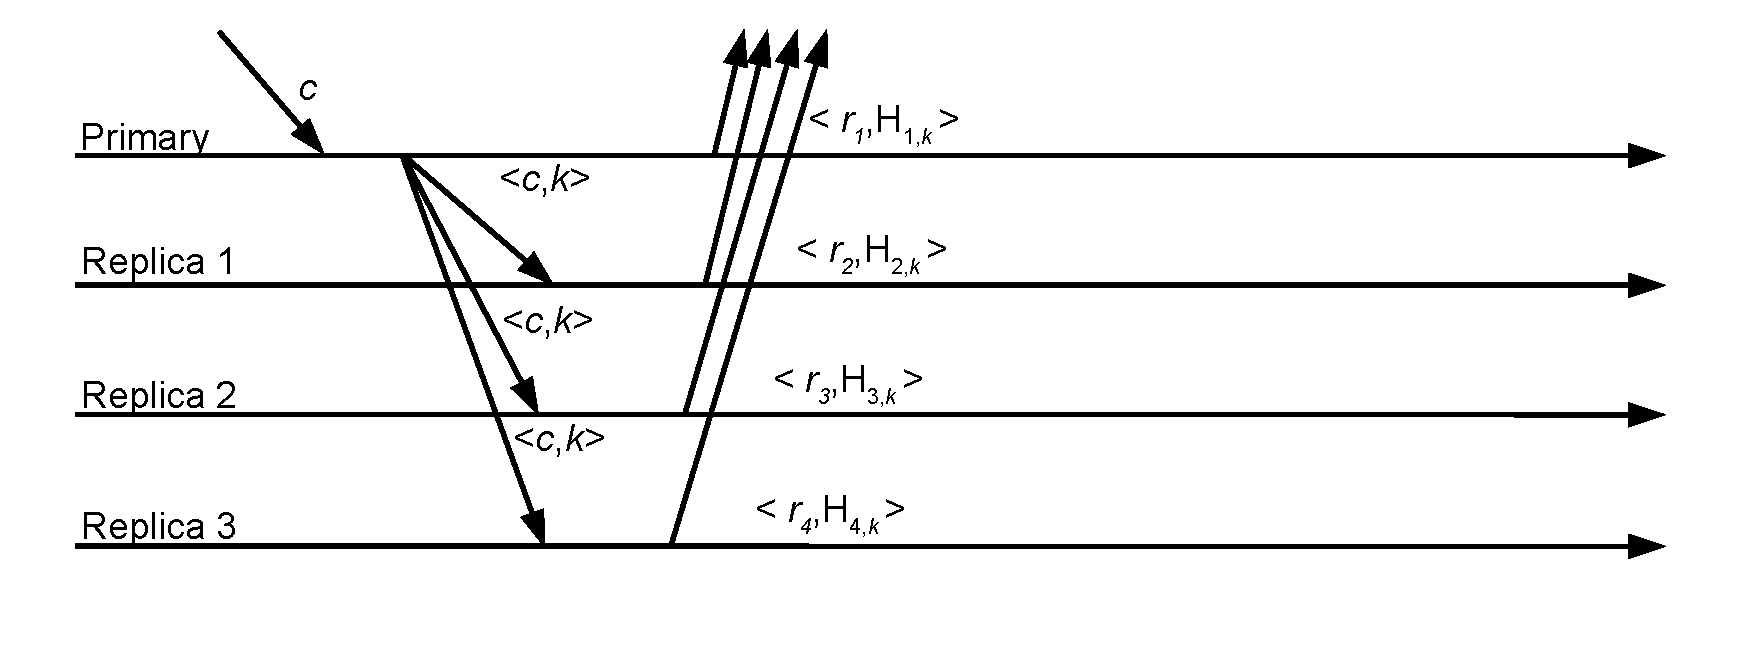
\includegraphics[width=\textwidth]{figs/17/messages6}	
\end{figure}

\BIL
\item Client processes response if all replies match:
\[
  r_1 = \ldots =r_ 4 \wedge H_{1,k} = \ldots = H_{4,k}
\]
\EIL

\end{frame}

\begin{frame}{Case 1: Unanimity}
	
Some comments:
\BI
\item Note that although a client has a proof that the request position
in the command history is irremediately set, no server has such a proof
\item Comparison of histories may be based on incremental hash
\item Three message hops to complete the request in the good case
\EI

\bigskip
Is it safe to accept the reply in this case?
\BI
\pause
\item All processes have agreed on ordering
\pause
\item Correct processes cannot change their mind later
\pause
\item New primary can ask $n-f$ replicas for their histories
\EI

\end{frame}

\begin{frame}{Case 2: A majority of correct replicas agree}

\begin{figure}
	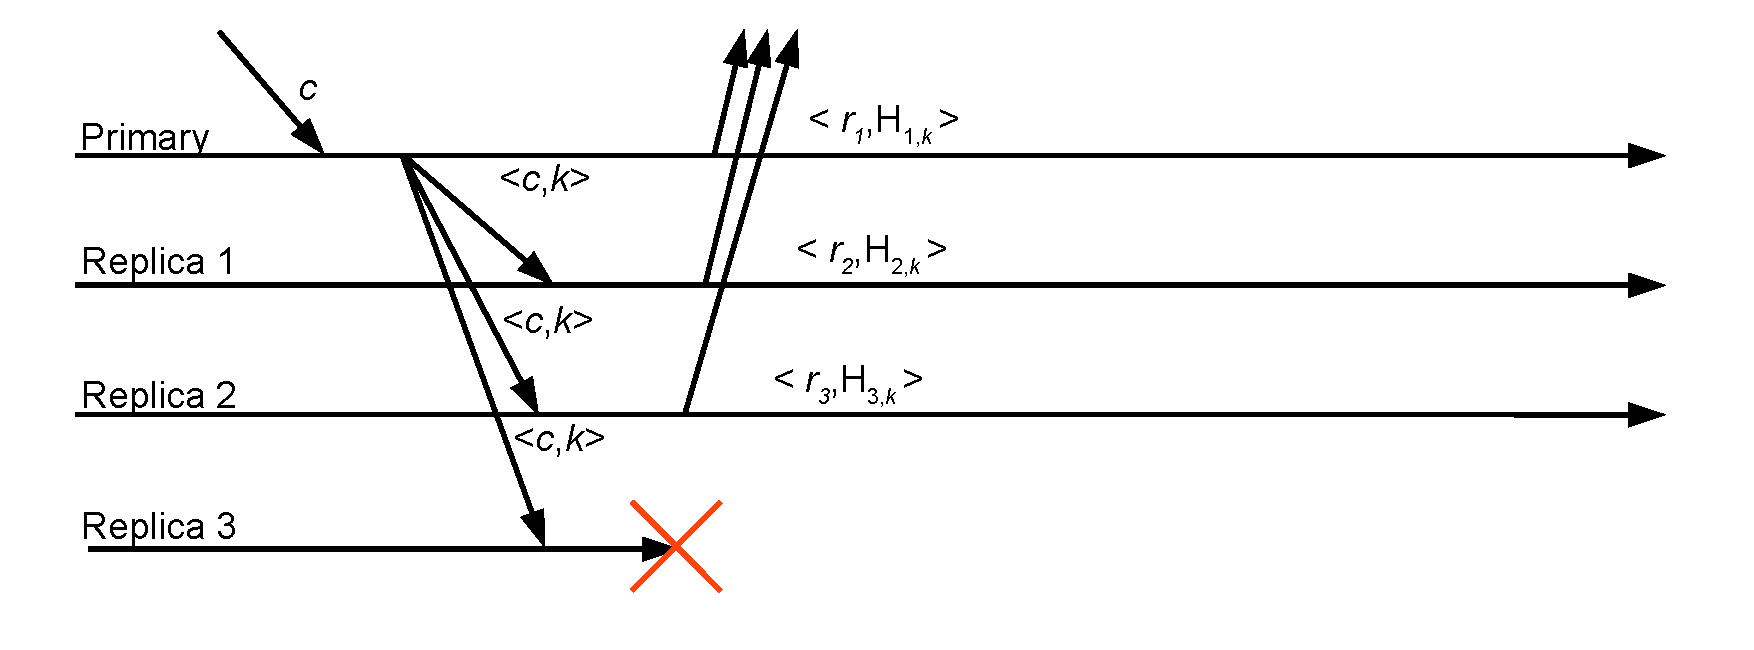
\includegraphics[width=\textwidth]{figs/17/messages7}	
\end{figure}

Is it safe to accept such a message?

\end{frame}

\begin{frame}{Case 2: A majority of correct replicas agree}

\begin{figure}
	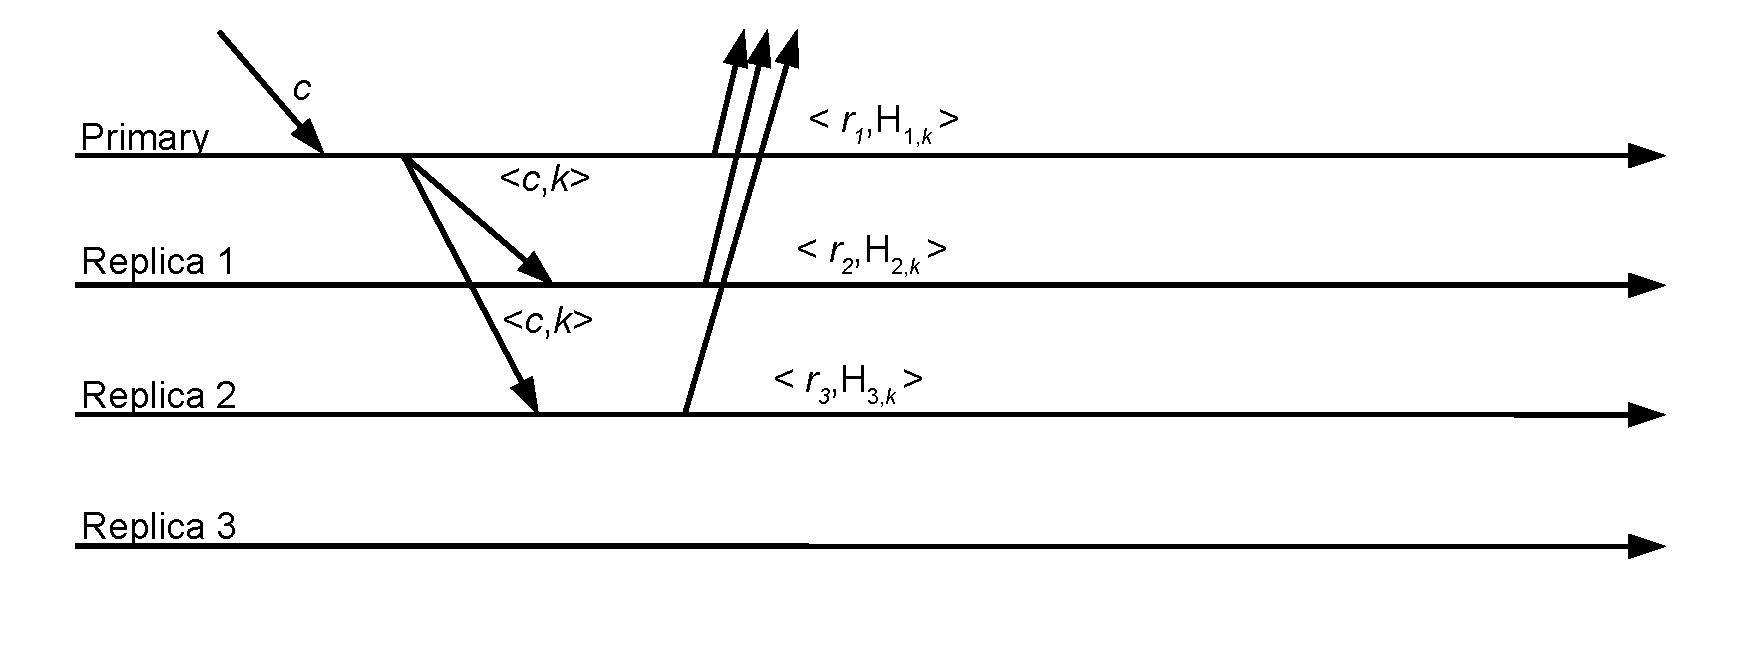
\includegraphics[width=\textwidth]{figs/17/messages8}	
\end{figure}

Consider this case...

\end{frame}

\begin{frame}{Case 2: A majority of correct replicas agree}

\begin{figure}
	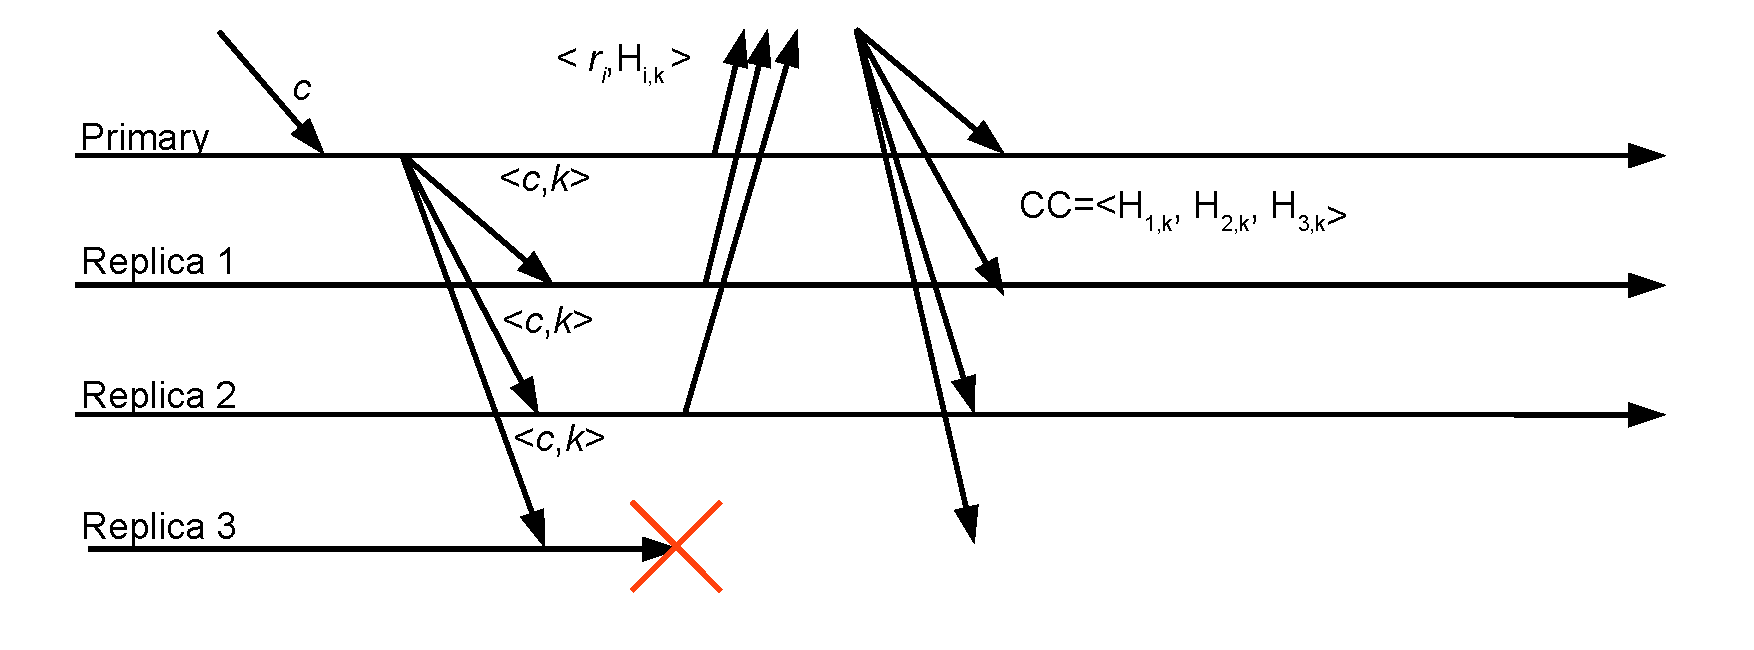
\includegraphics[width=\textwidth]{figs/17/messages9}	
\end{figure}

Client sends to all a \alert{commit certificate} containing $2f+1$ matching histories

\end{frame}

\begin{frame}{Case 2: A majority of correct replicas agree}

\begin{figure}
	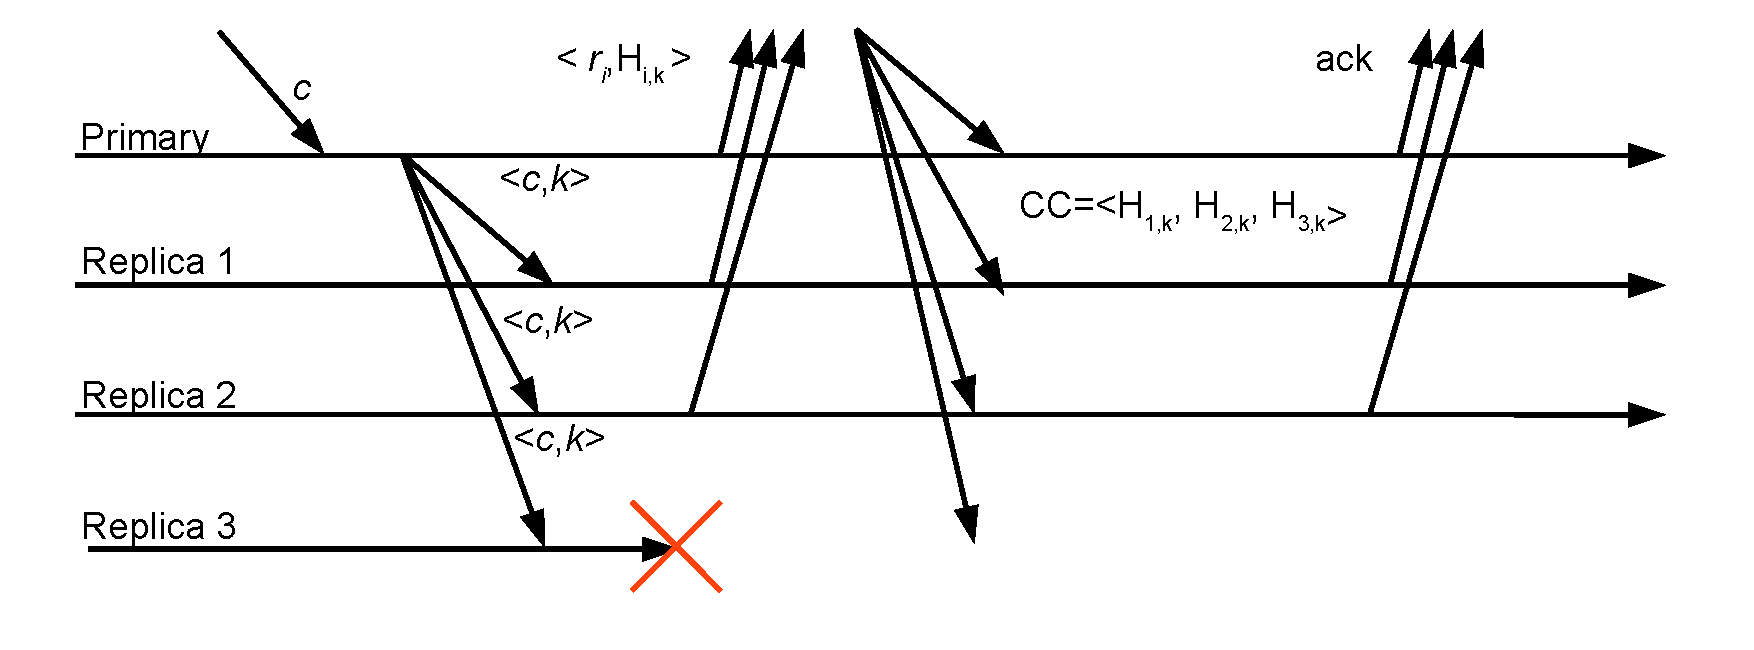
\includegraphics[width=\textwidth]{figs/17/messages10}	
\end{figure}

Client processes response if it receives at least $2f +1$ acks

\end{frame}

\begin{frame}{Case 2: A majority of correct replicas agree}
	
Safe?
\BIL
\item Certificate proves that a majority of correct processes agree on its position in the sequence
\item Incompatible with a majority backing a different command for that position
\EIL

\bigskip
Stability
\BIL
\item Stability depends on matching command histories 
\item Stability is \alert{prefix-closed}:
	\BI
	\item If a command with sequence number $k$ is stable, then so is every command with sequence number $k' < k$
	\EI
\EIL
\end{frame}

\begin{frame}{Case 3: None of the above}

\begin{figure}
	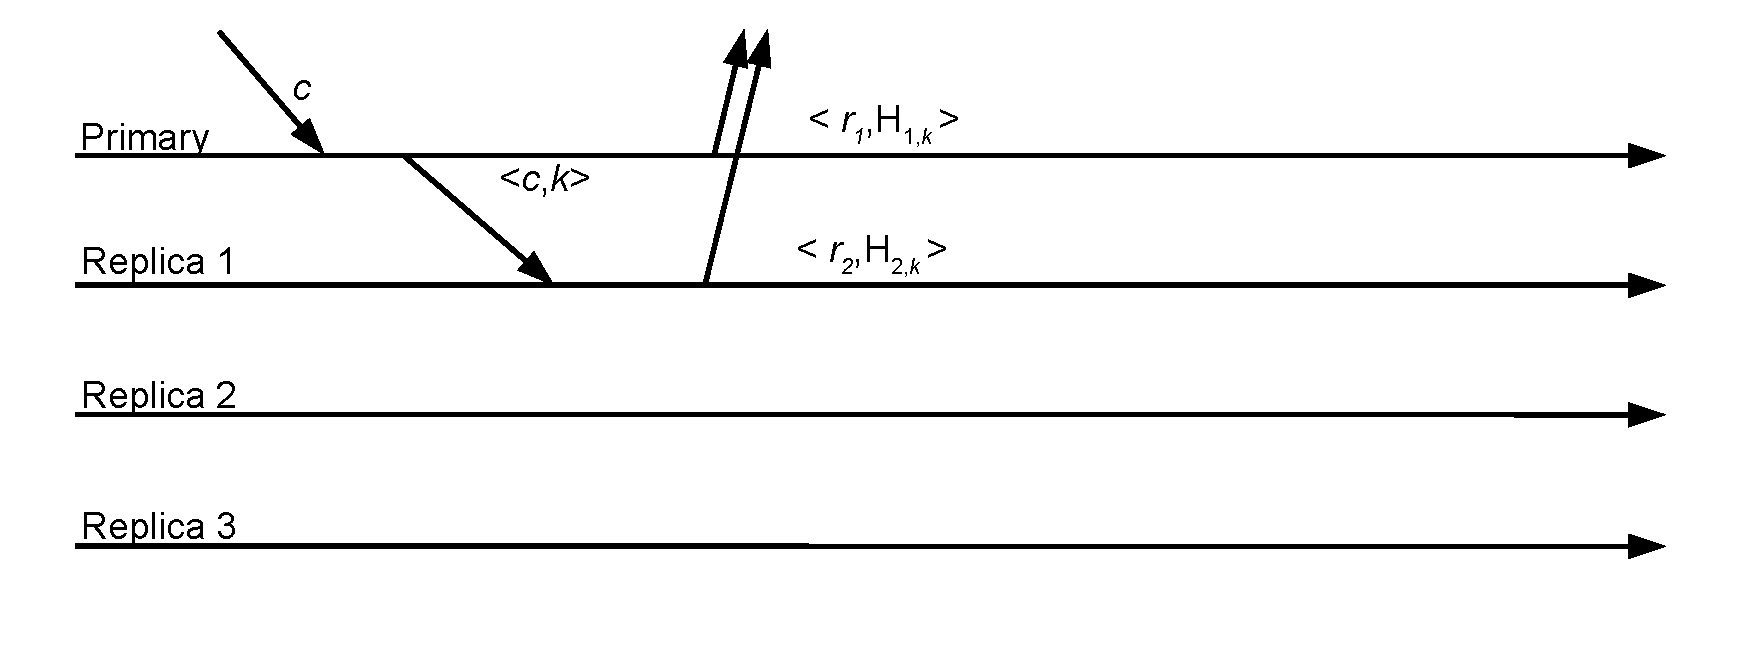
\includegraphics[width=\textwidth]{figs/17/messages11}	
	
\BIL
\item Fewer than $2f+1$ replies match
\item Clients retransmits $c$ to all replicas -- hinting primary may be faulty
\EIL	
	
\end{figure}

\end{frame}

\subsection{The case of the missing phase}

\begin{frame}{The case of the missing phase}

\begin{columns}
\begin{column}{0.6\textwidth}
\begin{figure}
	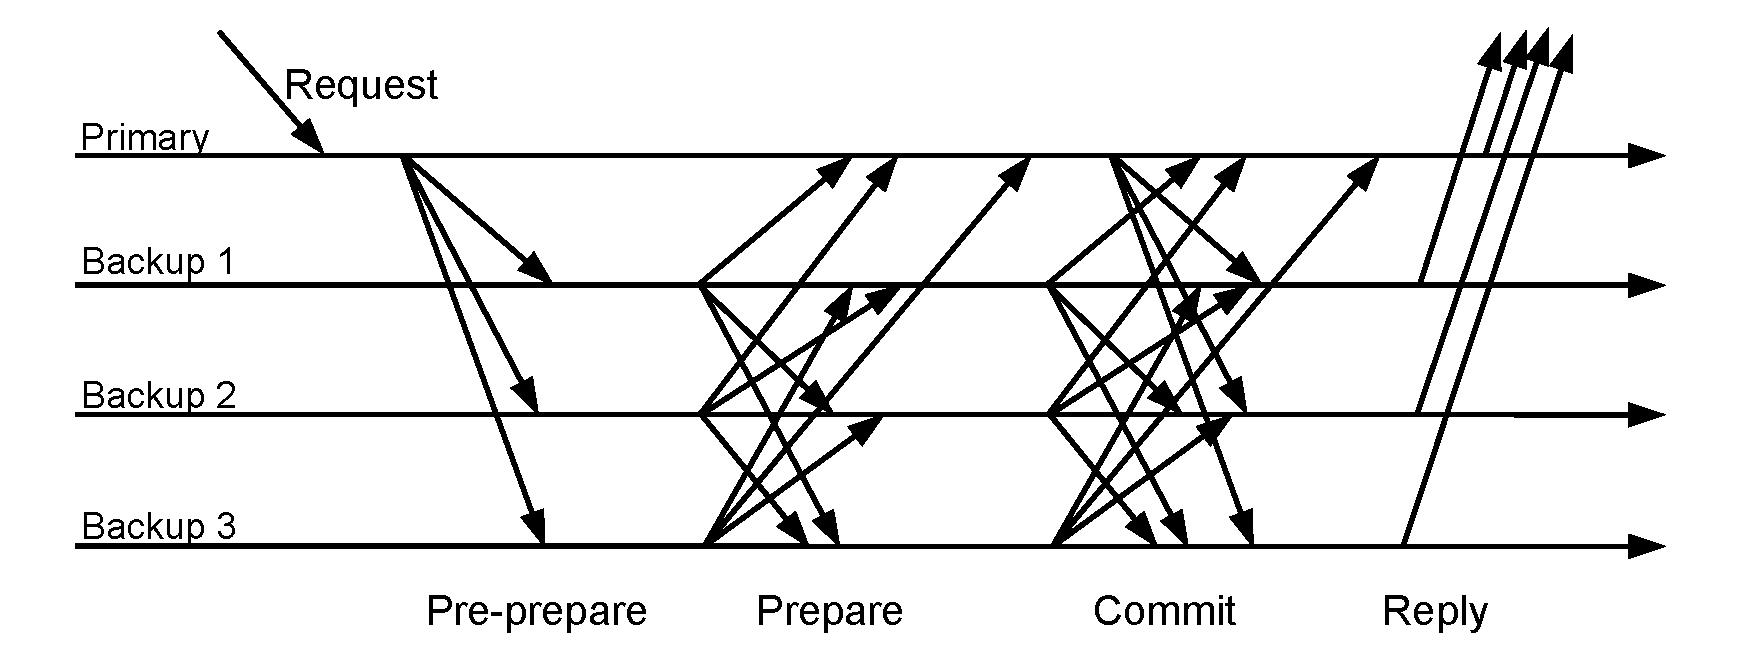
\includegraphics[width=\textwidth]{figs/17/messages4}
\end{figure}
\begin{figure}
	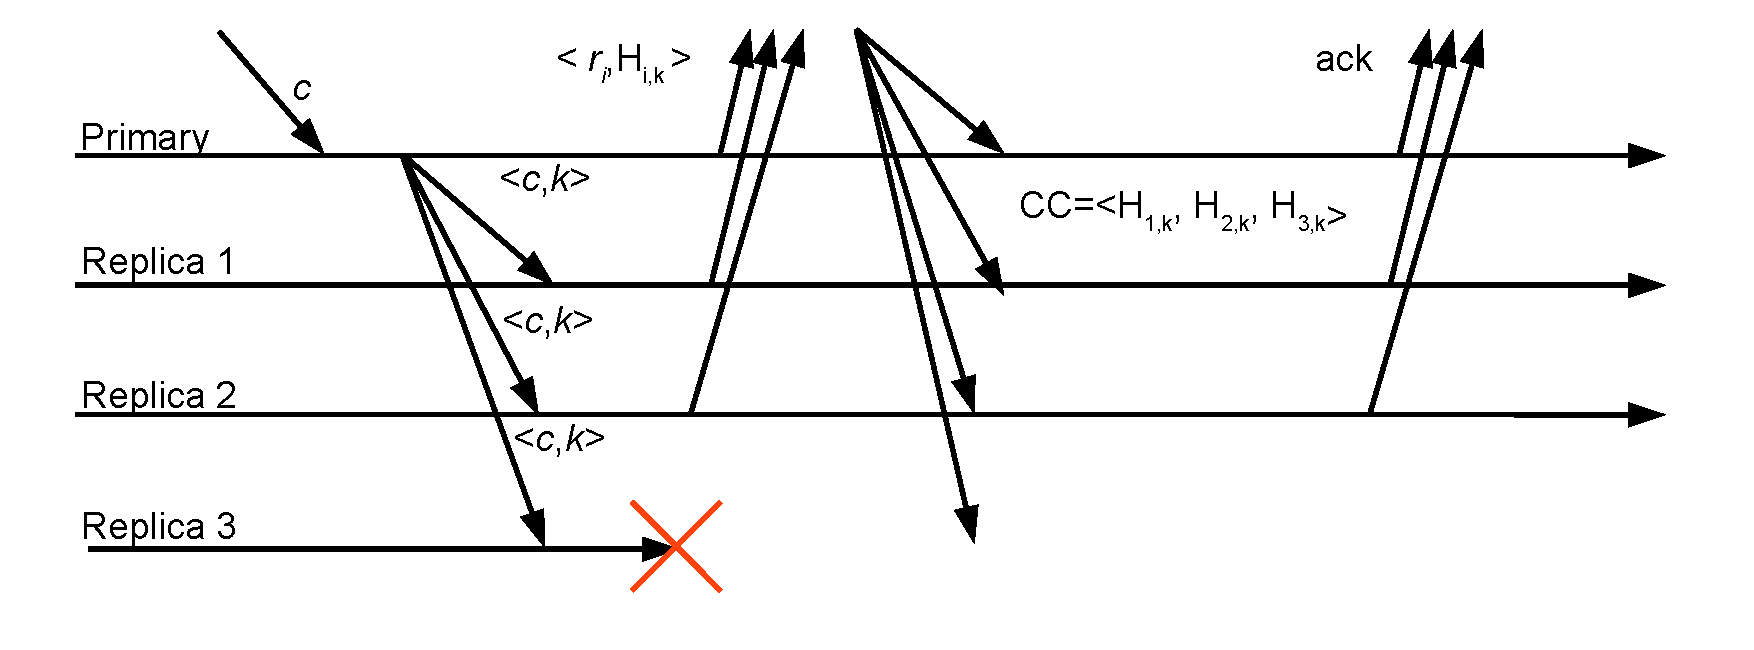
\includegraphics[width=\textwidth]{figs/17/messages10}	
\end{figure}
\end{column}
\begin{column}{0.4\textwidth}
\BIL
\item Where did the third phase go?
\item Why was it there to begin with?
\EIL	
\end{column}
\end{columns}
\end{frame}

\begin{frame}{The missing phase -- $\Commit$}
	
Consider this scenario:
\BI
\item $f$ malicious replicas, including the primary
\item The primary stops communicating with $f$ correct replicas
\item They go on strike -- they stop accepting messages in this view
\item $f+f$ replicas stops accepting messages, $f+1$ messages keep working
\item The remaining $f+1$ messages are not enough to conclude the $\Preprepare$ and
  $\Prepare$ phases
\item The $f$ correct processes that are asking a view change are not enough
  to conclude one, so there is no opportunity to regain liveness by electing
  a new primary
\EI
		
\end{frame}	

\begin{frame}{The missing phase -- $\Commit$}
	
The third phase of PBFT breaks this stalemate:
\BIL
\item The remaining $f+1$ replicas 
\BI
\item either gather the evidence necessary to complete the request,
\item or determine that a view change is necessary
\EI	
\item Commit phase needed for liveness
\EIL
	
\end{frame}

\subsection{View changes}

\begin{frame}{Where the third phase go?}
	
\begin{block}{In PBFT}
\begin{quote}	
What compromises liveness in the previous scenario is that the PBFT view
change protocol lets correct replicas commit to a view change and become
silent in a view without any guarantee that their action will lead to the view
change
\end{quote}
\end{block}

\begin{block}{In Zyzzyva}
\begin{quote}	
A correct replica does not abandon view $v$ unless it is guarantee that every
other correct replica will do the same, forcing a new view and a new primary
\end{quote}
\end{block}

\end{frame}

\begin{frame}{View change}
	
\BIL
\item Two phases:
\BI
\item Processes unsatisfied with the current primary sent a message
$\langle \textsc{i-hate-the-primary}, v \rangle$ to all
\item If a process collect $f+1$ \textsc{i-hate-the-primary} messages,
sends a message to all containing such messages and starts a new view
change (similar to the traditional one)
\EI
\item Extra phase of agreement protocol is moved to the view change protocol
\EIL
	
\end{frame}	

\begin{frame}{Optimizations}
	
\BIL
\item Checkpoint protocol to garbage collect histories 
\item Replacing digital signatures with MAC
\item Replicating application state at only $2f +1$ replicas
\item Batching
\EIL

\end{frame}

\begin{frame}{Performance}

\begin{figure}
	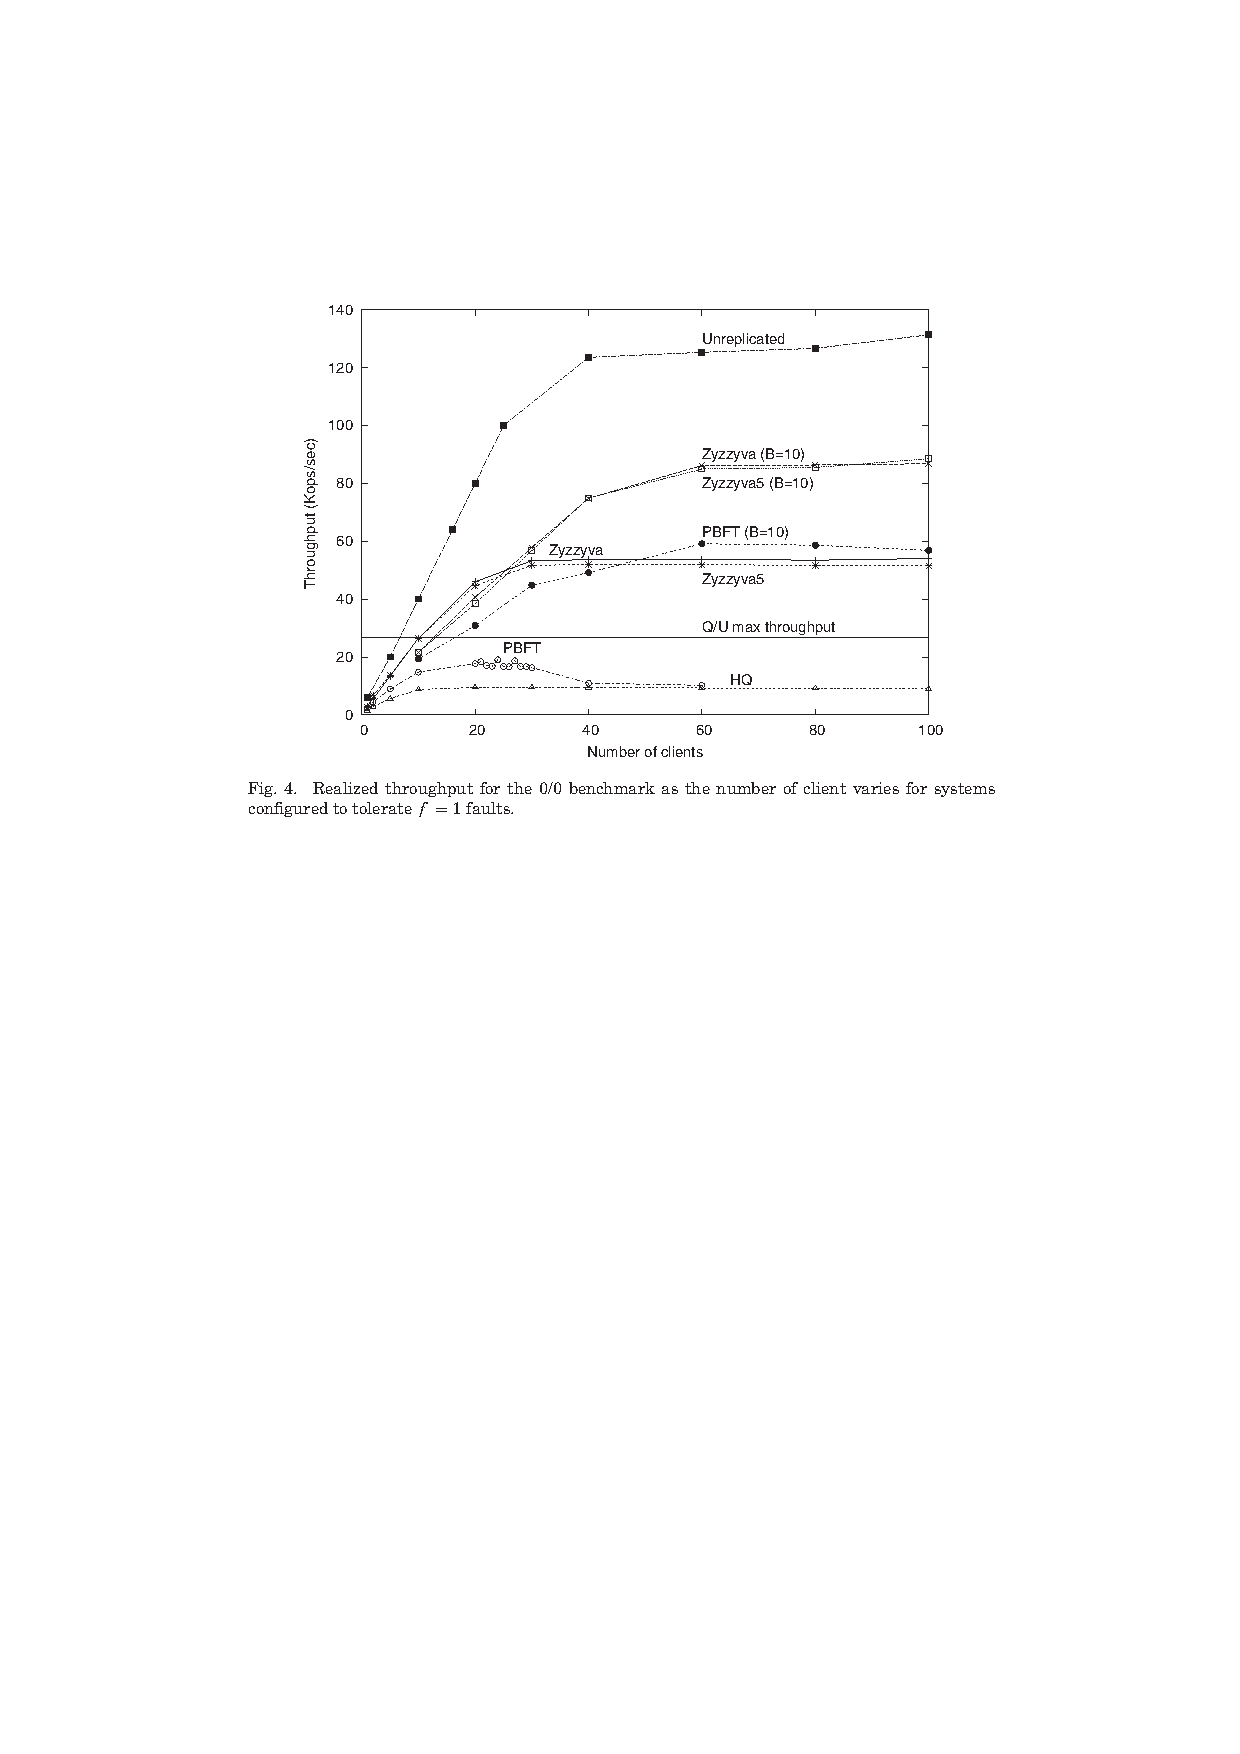
\includegraphics[width=0.8\textwidth]{figs/17/performance}
\end{figure}

\end{frame}

\begin{frame}{Discussion}

\BIL
\item What have you learned?
\item Do you agree on the principles?
\EIL
\end{frame}


\section{Aardvark}

\begin{frame}{Aardvark\footnote{Aardvark is the first word of the English dictionary}}
	
\begin{block}{NSDI'09}
{\small
\bibentry{aardvark}
}
\end{block}	
	
\begin{columns}
\begin{column}{0.4\textwidth}
\BIL
\item A new beginning!
\item {\tiny \url{http://en.wikipedia.org/wiki/File:Porc_formiguer.JPG}}

\EIL
\end{column}
\begin{column}{0.6\textwidth}
\begin{figure}
	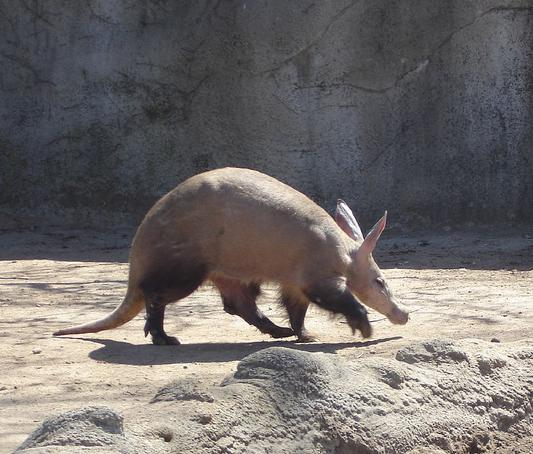
\includegraphics[width=0.5\textwidth]{figs/17/aardvark.png}\\
\end{figure}
\end{column}
\end{columns}

\note{+Oritteropo in Italian}

\end{frame}

\begin{frame}{From the article}

\begin{block}{Surviving vs tolerating}
\begin{quote}
Although current BFT systems can survive Byzantine faults without
compromising safety, we contend that a system that can be made completely
unavailable by a simple Byzantine failure can hardly be said to tolerate
Byzantine faults.
\end{quote}
\end{block}

\end{frame}

\begin{frame}{Conventional wisdom}
	
\begin{overprint}
\onslide<1|handout:1>
	\BIL
	\item Handle normal and worst case separately 
		\BI
		\item remain safe in worst case
		\item make progress in normal case
		\EI
	\EIL
\onslide<2-4|handout:2-4>
	\BIL
	\item Misguided
		\BI
		\item encourages systems that fail to deliver BFT
		\EI
	\EIL
\end{overprint}	
\bigskip
\begin{overprint}
\onslide<1-2|handout:1-2>
\BIL
\item Maximize performance when
	\BI
	\item the network is synchronous 
	\item all clients and servers behave correctly
	\EI
\EIL
\onslide<3-4|handout:3-4>
\BIL
\item Dangerous
	\BI
	\item it encourages \alert{fragile optimizations}
	\EI
\EIL
\end{overprint}
\onslide<4|handout:4>
\BIL
\item Futile
	\BI
	\item it yields \alert{diminishing return} on common case
	\EI
\EIL

\note{Go back to the previous slides on performance of the 0/0 case (null operation)}

\end{frame}

\begin{frame}{Blueprint}

\BIL
\item Build the system around execution path that:
\BI
\item provides acceptable performance across the broadest set of executions
\item it is easy to implement
\item it is robust against Byzantine attempts to push the system away from it
\EI
\EIL

\end{frame}	

\begin{frame}{Revisiting conventional wisdom}
	
\BIL
\item Signatures are expensive -- use MACs 
	\BI
	\item Faulty clients can use MACs to generate ambiguity 
	\item Aardvark requires clients to sign requests
	\EI
\item View changes are to be avoided
	\BI
	\item Aardvark uses regular view changes to maintain high throughput despite faulty primaries
	\EI
\item Hardware multicast is a boon
	\BI
	\item Aardvark uses separate work queues for clients and individual replicas	
	\item Aardvark uses fully connected topology among replicas
	  (separate NICs)
	\EI
\EIL	
\end{frame}

\begin{frame}{MAC Attack}

\begin{figure}
	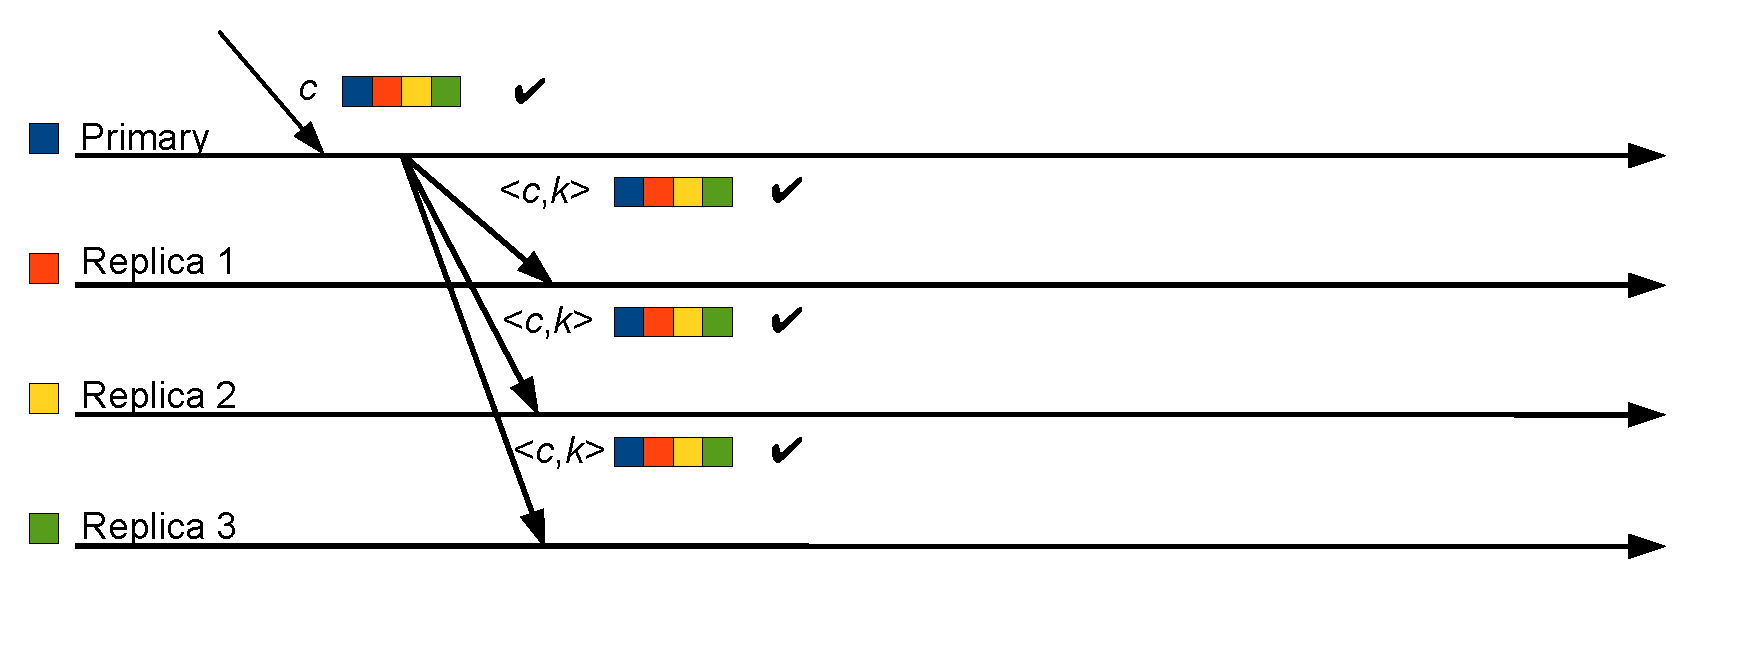
\includegraphics[width=\textwidth]{figs/17/messages12}\\
\end{figure}

\end{frame}

\begin{frame}{MAC Attack}

\begin{figure}
	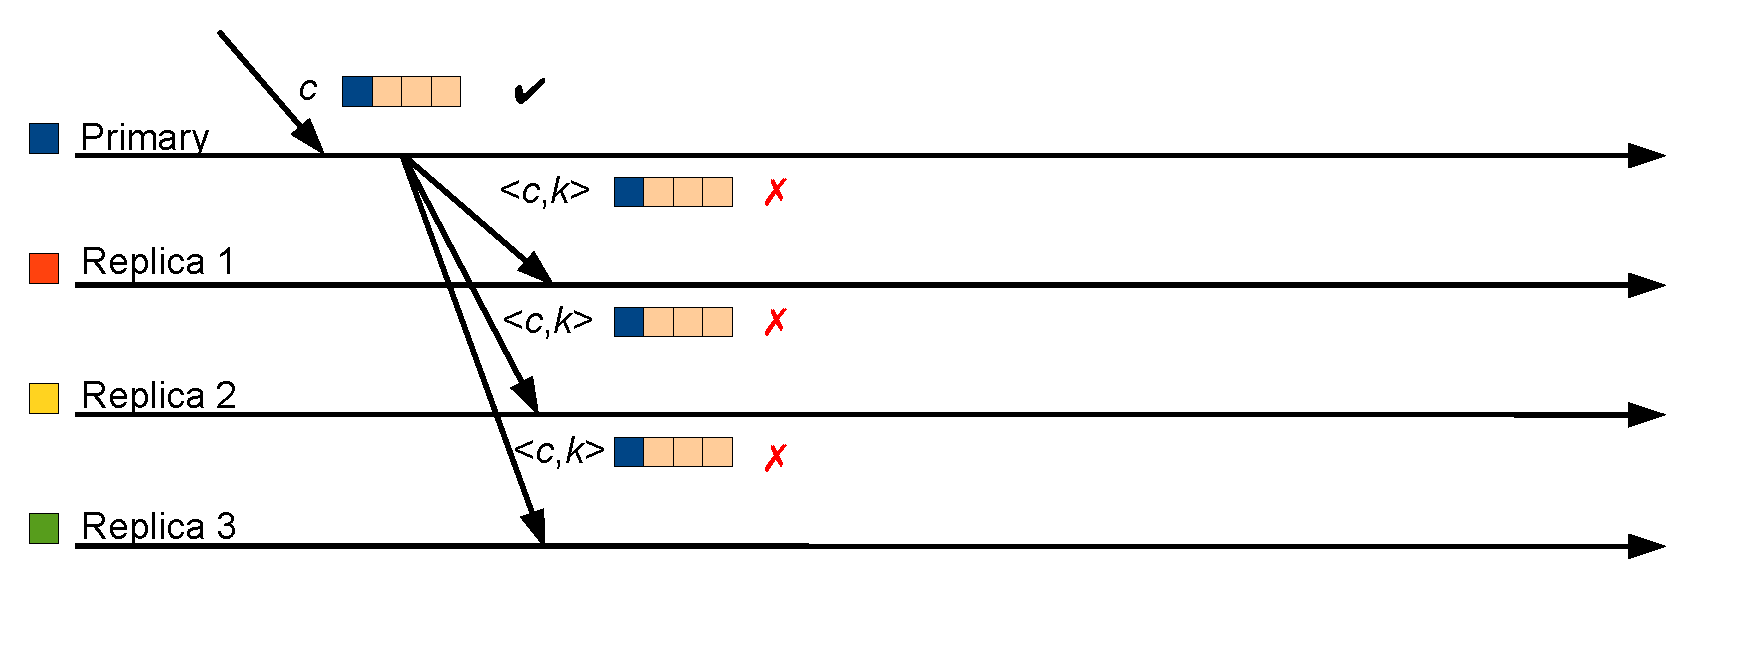
\includegraphics[width=\textwidth]{figs/17/messages13}\\
\end{figure}

\end{frame}

\begin{frame}{Throughput}

\begin{table}	
\begin{tabular}{|l|c|c|c|c|c|}
\hline
	& Best & Faulty & Client & Faulty & Faulty \\
	& case & client & flood	& primary & replica \\ \hline
PBFT & 62K & 0 & crash & 1k & 250 \\ \hline	
QU & 24K & 0 & crash & NA & 19k \\ \hline
HQ & 15K &	NA & 4.5K &	NA & crash \\ \hline
Zyzzyva & 80K &	0 & crash & crash & 0 \\ \hline
Aardvark & 39K & 39K & 7.8K	& 37K & 11K \\ \hline
\end{tabular}	
\end{table}
\end{frame}

\section{UpRight}

\begin{frame}{UpRight}

\begin{Bib}
\bibentry{upright}	
\end{Bib}

\BIL
\item A new (B)FT replication library
\item Minimal intrusiveness for existing apps 
\item Adequate performance 
\item Goal: 
	\BI
	\item ease BFT deployment 
	\item make explicit incremental cost of BFT 
	\item switching to BFT: simple change in a config file
	\EI
\EIL

\end{frame}

\begin{frame}{UpRight}
\BIL
\item $u$= max number of failures to ensure liveness
\item $r$ = max number of \alert{commission} failures to preserve safety
\EIL

\begin{columns}
\begin{column}{0.5\textwidth}
\begin{figure}
	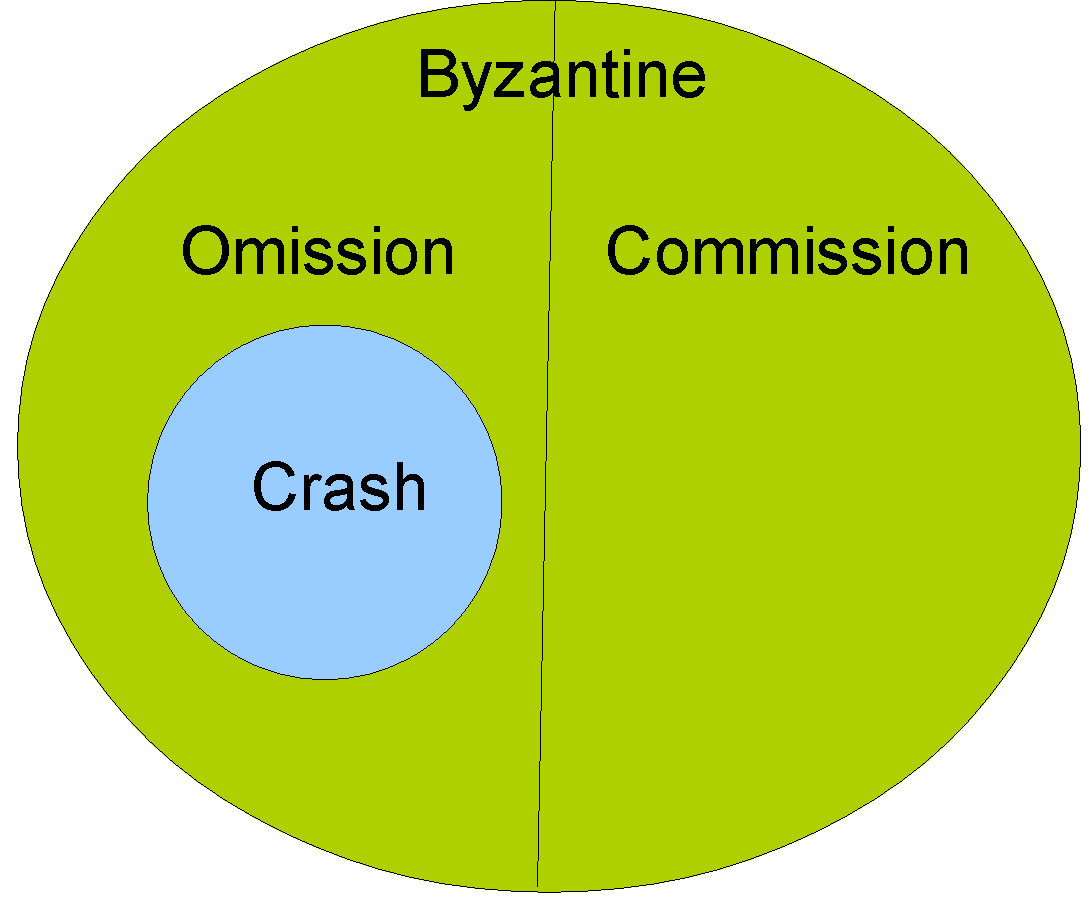
\includegraphics[width=\textwidth]{figs/17/commission}
\end{figure}
\end{column}
\begin{column}{0.5\textwidth}
\BIL
\item $r=u=f$: BFT 
\item $r=0$ : CFT	
\EIL 
	
\end{column}
\end{columns}
	
\end{frame}

\begin{frame}{UpRight}
\BIL
\item Exposes incremental cost of BFT
	\BI
	\item Byzantine agreement
	\item if $r << u$, BFT $\approx$ CFT in replication cost
	\EI
\item Allows richer design options
\BI
\item Byzantine faults are rare: $u > r$ 
\item Safety more critical than liveness: $r > u$
\EI
\EIL
\end{frame}


%%%%%%%%%%%%%%%%%%%%%%%%%%%%%%%%%%%%%%%%%%%%%%%%%%%%%%%%%%%%%%%%%%%%%%%%%%
\section{Bibliography}

%-------------------------------------------------------------------------
\begin{frame}{Reading material}

{\footnotesize
\BIL
\item \bibentry{zyzzyva}
\item \bibentry{aardvark}
\EIL
}

\invisible{{\tiny
\bibliographystyle{abbrv}
\bibliography{references} 
}}

\end{frame}

\end{document}